\newpage
\chapter{Additional improvements}

Since we observed that the computation time to solve hard instances significantly increased compared to easy instances, we decided to implement the improvements described in chapters 4 and 5 of Calik and Tansel (2013), i.e. the ``BINARY'' and one of the ``Double bound'' algorithms.
Actually, P3 is not even supposed to be solved with all variables $z_k$ with $k \in T$ since $T$ may have a very large cardinality.
Indeed, for every instance provided with the project statement, we noticed that there is very few redundancy in radius values, which makes set $R$ even larger.\\\\
Solving P3 reduces to selecting one of the values in $R$, which makes the value of the objective function equal to one of the values $\rho_k$ in $R$.
Indeed, each variable $z_k$ is associated to exactly one value $\rho_k$ in the objective function,
and exactly one variable $z_k$ must be selected. Thus, some of the values in $R$ can be discarded once we know either an upper bound $UB$ or a lower bound $LB$.
More specifically, all values $\rho_k < LB$ and all values $\rho_k > UB$ can be removed from the problem.\\\\

\section{BINARY algorithm}

BINARY algorithm is not the fastest method for dropping indices from $\{1, 2, \ldots, |T|\}$, but is quite easy to implement.
It is basically a bisection search on the optimal value of the objective function for the linear relaxation of Px (P2, P3 or P4).\\\\
Let:
\begin{itemize}
	\item LPx denote the relaxation of Px
	\item val(LPx) denote the optimal value of Px.
	\item RPx denote the relaxation that retain the objective function and all constraints of Px
	\item $P_h$ with $h \in T$ be the problem P3 with the additional constraint $z_h = 1$
	\item $RP_h$ with $h \in T$ be the problem RP3 with the additional constraint $z_h = 1$
	\item val($P_h$) be the optimal value of $P_h$
	\item val($RP_h$) be the optimal value of $RP_h$
\end{itemize}\ \\
Calik and Tansel (2013) proposes and proves that val($RP3$)$ = \min_{h \in T}$ val($RP_h$). They show that computing $\min_{h \in T}$ val($RP_h$) is achieved in polynomial time by solving $\mathcal{O}\left( \log_2 K \right)$ linear programs $RP_h$ for each $\rho_h$ selected from the set of ordered $\rho$ values $R = \lbrace \rho_1, \rho_2, ..., \rho_K \rbrace$ (as defined in P3) during a binary seach.\\\\
The BINARY algorithm proposed by Calik and Tansel (2013) can be schematized as follows:
\begin{figure}[h!]
	\begin{center}
		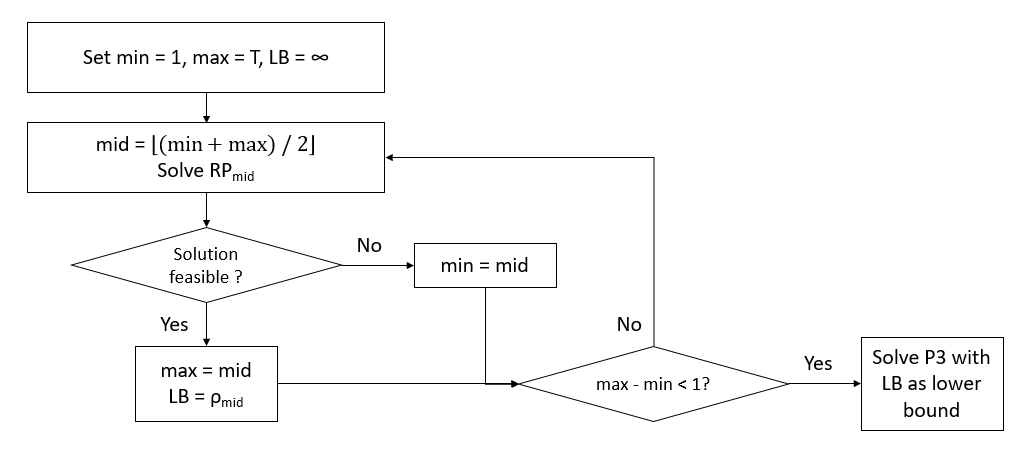
\includegraphics[width=\textwidth]{../imgs/BINARY.png}\\
		Flow chart of BINARY algorithm
	\end{center}
\end{figure}
\noindent Applying a bisection search on the objective function of the linear relaxation comes to the same as applying a bisection search
on the objective function of the original problem. Indeed, an integer problem is infeasible if there is an infeasible relaxation of this problem.
Thus, the algorithm stops once the feasible solution with the lowest value of the objective has been found. \\\\
In our actual implementation we stop iterating once $max - min < 2$ because we consider that solving the primal problem for two indices from $T$ is faster
than running an additional linear relaxation before running the primal on a unique index $mid$.
This idea is also inspired by DB algorithms described in next section.\\\\
The main defect of this method is that it cannot be used alone, since it does not provide any upper bound.
Instead of combining BINARY with another technique for finding $UB$, we decided to implement one of the
double bound (DB) methods for the purpose of diversification among the algorithms discussed.
\section{Double bound algorithm}
Since comparing performance for different DB algorithms is not part
of the present project's objective, we only implemented one of them (that we did not assume to be the fastest
one). However, DB3 was reported in the paper to terminate in $\mathcal{O}(\log_3 T)$ iterations (against $\mathcal{O}(\log_2 T)$ iterations for DB1 and DB2).\\\\
Let:
\begin{itemize}
	\item $S$ be any nonempty subset of $T = \lbrace 1, ..., K \rbrace$
	\item $P(S)$ be the problem which is exactly the same as P3 except that all variables $z_k, k \in T\\S$ are dropped from P3
\end{itemize}\ \\
Calik and Tansel (2013) proposes and proves the following:\\\\
``Suppose $|S| > 2$. Let a and b be the smallest ad largest indices in S, respectively.\\
\begin{tabularx}{\textwidth}{l X}
(a) & If val($P(S)$) = $\rho_a$, then $r_p(F) \in \lbrace \rho_1, ..., \rho_a \rbrace$\\
(b) & If val($P(S)$) = $\rho_k$ for some $k$ with $a < k \leq b$, then $r_p(F) \in \lbrace \rho_{k'+1}, ..., \rho_k \rbrace$ where $k'$ is the largest index in $S$ which is smaller than $k$ \\
(c) & If val($P(S)$) = $\infty$, then $r_p(F) \in \lbrace \rho_{b+1}, ..., \rho_K \rbrace$''\\
\end{tabularx}\ \\\\
This proposition allows the construction of a more efficient search strategy based on the restriction of P3. 
Unfornately, the paper of Calik and Tansel (2013) made no mention of the feasibility of problem $P(S)$.
Indeed, with small values for both $\rho_a$ and $\rho_b$, $P(\{\rho_a, \rho_b\})$ may be infeasible.
This occurs when both $\rho_a$ and $\rho_b$ values are below the lowest objective value among feasible $RP_h$ solutions.
As a result, $P(S)$ may be infeasible for a certain set $S$ in exactly the same way that $RP_h$ may be infeasible for a certain index $h$.
For that reason, we set $min = b + 1$ if $P(S)$ is feasible, since both $a$ and $b$ would have led to an infeasible solution in BINARY algorithm.
In other words, all radius values less or equal to $\rho_b$ (> $\rho_a$) are discarded from the search space.
The double bound algorithm proposed by Calik and Tansel (2013) can now be schematized as follows:
\begin{figure}[h!]
	\begin{center}
		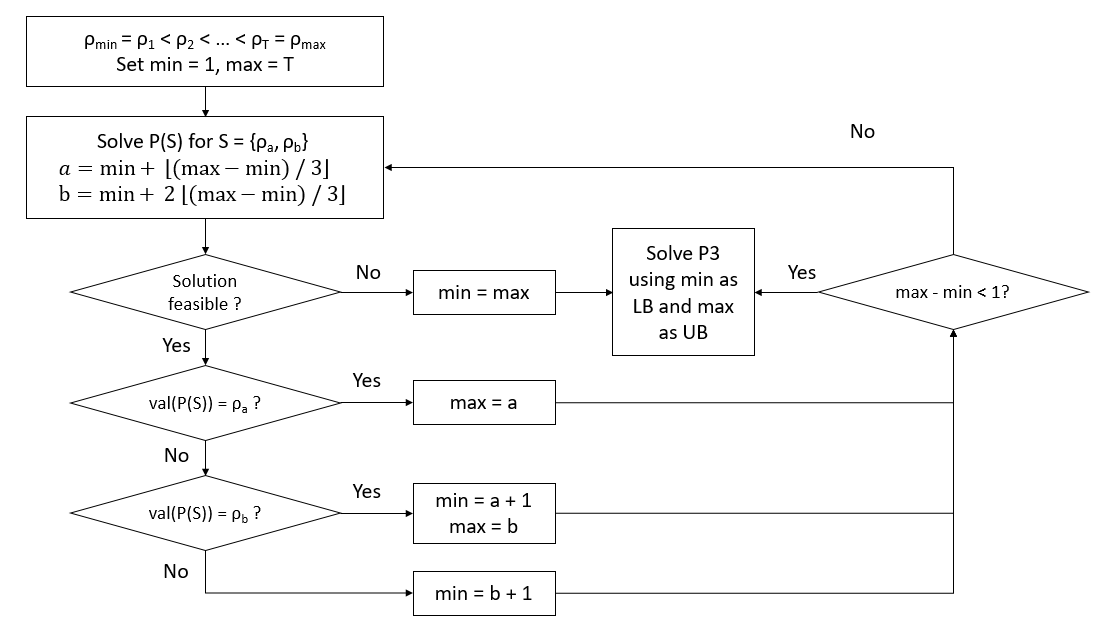
\includegraphics[width=\textwidth]{../imgs/DB3.png}\\
		Modified flow chart of DB3 algorithm
	\end{center}
\end{figure}